\documentclass[tikz, border=10pt]{standalone}
\usepackage{tikz}
\usepackage{amsmath}
\usetikzlibrary{shapes, arrows.meta, positioning, calc}

% The practitioner recipe of the conclusion as a decision flow.
\begin{document}
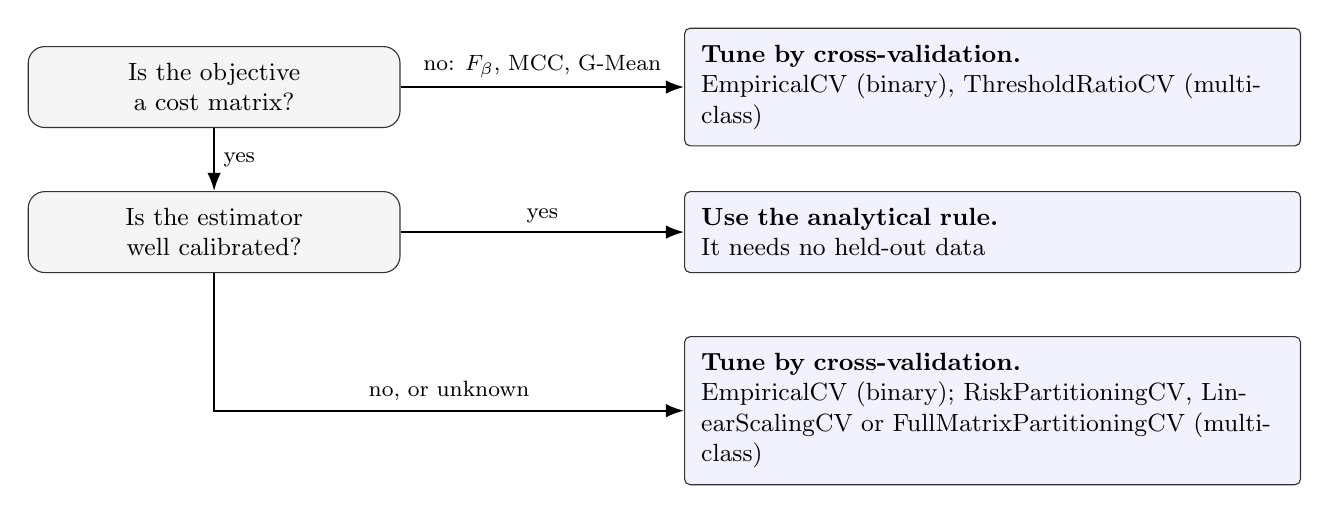
\begin{tikzpicture}[
    node distance=0.8cm and 3.6cm,
    ask/.style={rectangle, draw=black!80, fill=gray!8, rounded corners=6pt,
      font=\small, align=center, inner sep=6pt, text width=4.3cm},
    act/.style={rectangle, draw=black!80, fill=blue!5, rounded corners=2pt,
      font=\small, align=left, inner sep=6pt, text width=7.4cm},
    line/.style={draw, -Latex, thick},
    edgelbl/.style={font=\footnotesize, inner sep=3pt}]

  \node[ask] (obj) {Is the objective a cost matrix?};
  \node[ask, below=of obj] (cal) {Is the estimator well calibrated?};

  \node[act, right=of obj] (metric)
    {\textbf{Tune by cross-validation.}\\
     EmpiricalCV (binary), ThresholdRatioCV (multiclass)};
  \node[act, right=of cal] (ana)
    {\textbf{Use the analytical rule.}\\ It needs no held-out data};
  \node[act, below=of ana] (cost)
    {\textbf{Tune by cross-validation.}\\
     EmpiricalCV (binary); RiskPartitioningCV, LinearScalingCV or
     FullMatrixPartitioningCV (multiclass)};

  \path[line] (obj) -- node[edgelbl, above] {no: $F_\beta$, MCC, G-Mean}
    (metric);
  \path[line] (obj) -- node[edgelbl, right] {yes} (cal);
  \path[line] (cal) -- node[edgelbl, above] {yes} (ana);
  \path[line] (cal) |- node[edgelbl, pos=0.75, above] {no, or unknown}
    (cost);
\end{tikzpicture}
\end{document}
